\documentclass[../TV&MS.tex]{subfiles}
\begin{document}
    
\section{Виды распределений}

Распределения случайных величин можно разделить на 3 типа: непрерывные, дискретные и сингулярные.

\begin{Def}
	Случайная величина $\xi$ называется \underline{абсолютно непрерывной}, если существует интегрируемая функция $p_\xi(x) \ge 0, \ x \in \Real$ такая, что
	функция распределения $\xi$ является почти всюду (за исключением не более, чем счетного числа точек) дифференцируемой функцией и представима в виде
	$$F_\xi(x) = \int\limits_{-\infty}^x p_\xi(y)dy$$
	Отсюда следует, что функция распределения непрерывна на $\Real$. $p_\xi(x)$ называется \underline{плотностью распределения},
	и почти всюду выполнено $p_\xi(x)=F_\xi'(x)$.
	Плотность, вообще говоря, определена не однозначно.
\end{Def}

\begin{Def}
	Случайная величина $\xi$ называется \underline{дискретной}, если множество точек роста не более, чем счетно, но распределение не является сингулярным, или, 
	другими словами $\exists B = \{x_1, x_2, \ldots\} \colon \Pro(\xi \in B) = 1$.
\end{Def}

\begin{Def}
	Случайная величина $\xi$  называется \underline{сингулярной}, если $F_\xi$ непрерына, и $\exists B \in \Bor \colon \mu(B) = 0, \ \Pro(\xi \in B) = 1$, то есть множество значений случайной величины имеет меру 0, но вероятность попасть в каждую точку этого множества так же нулевая.
\end{Def}

Пара слов о жизненном смысле определений: непрерывная случайная величина имеет областью значений континуальное множество, при этом вероятность попасть в отдельно взятую точку нулевая. Пример: равномерное распределение по отрезку. Плотность же отражает вероятность попасть в ту или иную область: интеграл по области равен этой вероятности. Дискретная случайная величина принимает конечное или счетное множество значений, вследствие этого имеет ступенчатую функцию распределения, например, бросок монетки имеет дискретное распределение. Сингулярное распределение --- это крокодил, который 
не встречается в жизни и будет рассмотрен отдельно.

\begin{St}
	Дискретная случайная величина имеет не более, чем счетное число скачков.
\end{St}
\begin{Proof}
Из свойств функции распределения следует, что дискретная величина имеет не больше двух скачков величины больше $\frac12$. Аналогично, скачков величины больше $\frac13$ не больше 3. То есть скачков величины больше $\frac1n$ не более n. Для любого скачка можно указать $n \in \mathbb{N}$ такое, что величина, этого скачка больше 
$\frac1n$. Значит,каждому скачку можно поставить в соответствие $n$, множество которых счетно. При этом для каждого $n$ существует не более чем счетное число скачков, ему соответсвующих (величины $>\frac1n$). А так как объединение не более, чем счетного числа не более, чем счетных множеств, не более, чем счетно, получаем 
требуемое. 
\end{Proof}

\begin{Ex}
Для полного счастья приведем пример сингулярной случайной величины. Пусть функция распределения - так называемая лестница Кантора (см. рисунок).
\parbox[b][3 cm][t]{20mm}{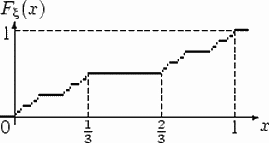
\includegraphics[height=30mm]{kantor}}
\hfill
\parbox[b][3 cm][t]{100mm}{
	Посчитаем меру множества, на котором функция константа, то есть точки этого множества не будут точками роста: сначала это одна ступенька длины 1/3, потом две длины 1/9, и т.д.

}\\
	$$ \frac13 + \frac29 + \frac4{27} = \frac13 \sum\limits_{k=1}^\infty(\frac23)^{k-1} = 1$$
	Тогда множество точек роста имеет меру 0 в силу свойства аддитивности меры.
\end{Ex}

Вообще говоря, существуют менее изысканные примеры сингулярных распределений. Например, при стрельбе из лука в круглую мишень распределение будет сингулярным,
если стрелок попадает только в точки одной прямой. В самом деле, двумерная мера прямой равна 0, как и вероятность попасть в каждую отдельную точку. 

\begin{Th} [Лебега]
	Любую случайную величину можно представить в виде суммы дискретной, абсолютно непрерывной и сингулярной случайной величины. То есть 
	$$ F(x) = \alpha_dF_d(x) + \alpha_cF_c(x) + \alpha_sF_s(x), \quad \alpha_d + \alpha_c + \alpha_s = 1$$
\end{Th}
\begin{Proof}
вышло и не вернулось
\end{Proof}

\newpage


\end{document}
